\documentclass[11pt]{article}

\usepackage{graphicx}
\usepackage{hyperref}
\usepackage{natbib}
\usepackage{amsmath}

\bibliographystyle{plain}
\setlength{\textwidth}{6.5in}
\setlength{\headheight}{0in}
\setlength{\textheight}{8.0in}
\setlength{\hoffset}{0in}
\setlength{\voffset}{0in}
\setlength{\oddsidemargin}{0in}
\setlength{\evensidemargin}{0in}


\title{Computational Physics -  Problem Set 5}
  
\author{Frederik Holst Knudsen}


\begin{document}

\maketitle
Github URL: https://github.com/frederikholst/phys-ga2000
\section{Newman 5.15}
We use the central difference method to compute the derivative of $1+\frac{1}{2}\tanh(2x)$. The result is compared in Figure \ref{cent} against the analytic derivative, $\sec^2(2x)$. In Figure \ref{jax} we see the same comparison, but with the JAX method instead of the central limit derivative method.
\begin{figure}[!htbp]
    \centering
    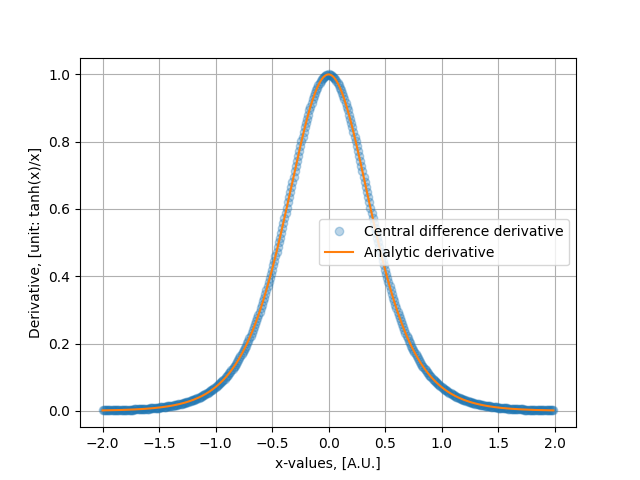
\includegraphics[width=0.7\textwidth]{problem1.png}
    \caption{The analytic derivative is plotted against the numerically computed derivative using central difference method. We see very good agreement.}
    \label{cent}
\end{figure}
\begin{figure}[!htbp]
    \centering
    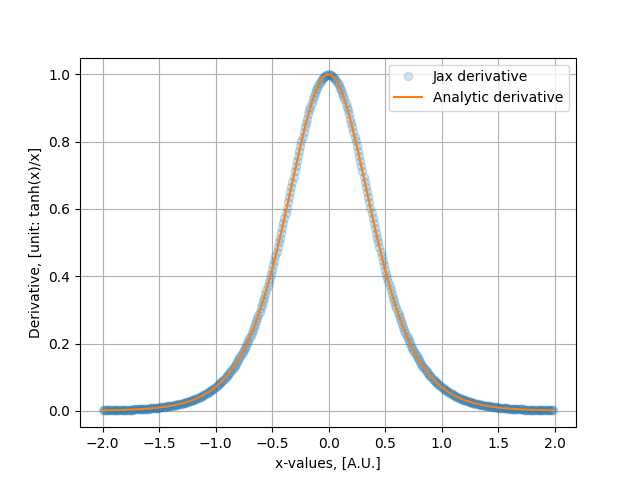
\includegraphics[width=0.7\textwidth]{Jax.png}
    \caption{The analytic derivative is plotted against the derivative using JAX. Again, we see very good agreement.}
    \label{jax}
\end{figure}

Finally, Figure \ref{resid} shows the residuals that are the size of machine errors.

\begin{figure}[!htbp]
    \centering
    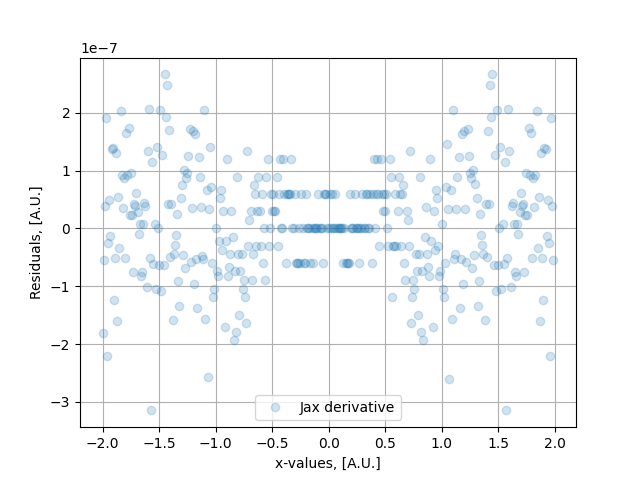
\includegraphics[width=0.7\textwidth]{Jax_res.png}
    \caption{The residuals are very small, which confirms that the JAX derivative is a strong method for computing the derivatives.}
    \label{resid}
\end{figure}

\section{Newman 5.17}


Part A: In Figure \ref{integrand} we see the integrand of the gamma function, $\Gamma(a)=\int_{0}^{\infty}x^{a-1}e^{-x}$ plotted for $n=2,3,4$.

\begin{figure}[!htbp]
    \centering
    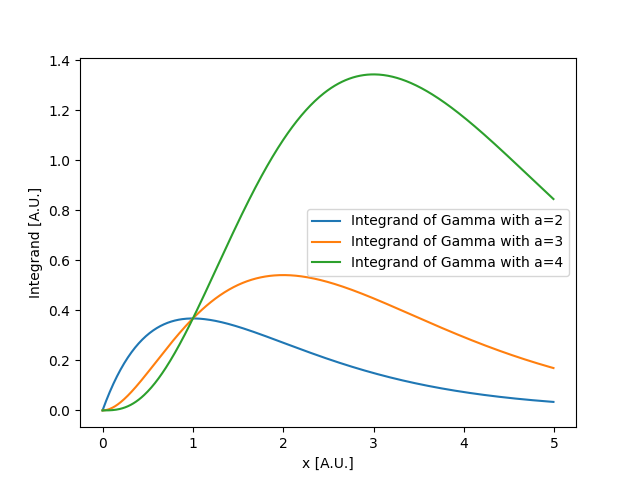
\includegraphics[width=0.7\textwidth]{integrand_plot.png}
    \caption{The integrand of the gamma function.}
    \label{integrand}
\end{figure}


Part B: 
We now show analytically that the maximum of the integrand falls at $x=a-1$. 

$$\frac{d}{dx}x^{a-1}e^{-x}=e^{-x}((a-1)x^{a-2}-x^{a-1})=0$$
$$\Rightarrow ax^{a-2}-x^{a-2}-x^{a-1}=0$$
$$\Rightarrow x^{a-2}(a-1-x)=0$$
$$\Rightarrow x_{max}=a-1$$


Part C:
Knowing that most of the integral will fall around $x_{max}=a-1$, we perform a change of variables using 
$$z=\frac{x}{c+x}$$ 
if $z=\frac{1}{2}$ at the maximum then $x_{max}=c$ so that
$$c=a-1$$.
And the variable change becomes:
$$z=\frac{x}{c+x}$$
$$\Rightarrow (c+x)z=x$$
$$\Rightarrow (zc=x(1-z))$$
$$\Rightarrow x=\frac{zc}{1-z}$$
$$\Rightarrow x=\frac{z(a-1)}{1-z}$$



Part D:
We will now write $x^{a-1}=e^{(a-1)\ln{x}}$ in the integrand of the gamma function. The new expression is better that the old one, because $x^{a-1}$ can easily cause overflow, and the new form puts two exponential functions in the integrand: $e^{(a-1)\ln{(x)}-x}$. This avoids the issue of having a very large number multiplied with a very small one, where both could be in the danger of overflow and underflow. 

Part E:
We now compute the gamma function using the change of variables:
$$\frac{dx}{dz}=\frac{(a-1)}{1-z}+\frac{z(a-1)}{(1-z)^2}$$

$$\Rightarrow \frac{dx}{dz} =\frac{z(a-1)-(a-1)(z-1)}{(1-z)^2}$$
$$\Rightarrow \frac{dx}{dz} =\frac{za-z-za+a+z-1}{(1-z)^2}$$
$$\Rightarrow \frac{dx}{dz} =\frac{a-1}{(1-z)^2}$$

So that the integral becomes:
$$ \Gamma (n)= \int_{0}^{1}dz\left(\frac{(a-1)}{1-z}+\frac{z(a-1)}{(1-z)^2}\right) \exp \left[ {(a-1)\ln{\left(\frac{z(a-1)}{1-z}\right)}-\frac{z(a-1)}{1-z}}\right]$$



We will use the gauss-quadrature method, and find the $\Gamma(\frac{3}{2}=0.8862272081548225)$ at 50 sample points in the Guass-quadrature integration. If we compare to the analytic value of $\frac{1}{2}\sqrt{\pi}=0.886$, we see very strong agreement. 

Part F:
Computing  $\Gamma(a)$ with interger values of $a$ replicates that of the theoretical analytic values $a-1!$ with strong precision: 
$$\Gamma(3)= 2.000000000000057, (3-1)!=2$$
$$\Gamma(6)=  119.99999999999946, (6-1)!=120$$
$$\Gamma(10)= 362879.99999999825, (10-1)!=362880$$


\section{Problem 3}
Part A: We import  plot the data as seen in Figure \ref{time_series}. 

\begin{figure}[!htbp]
    \centering
    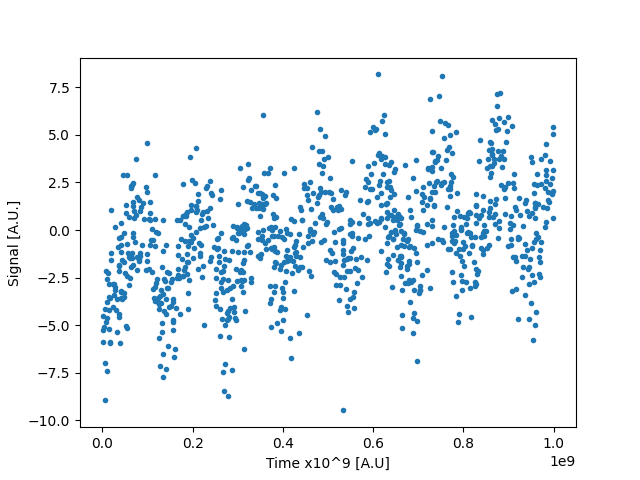
\includegraphics[width=0.7\textwidth]{time_series.png}
    \caption{The noisy signal is shown with normalized time. This will make approximation erros less likely later on.}
    \label{time_series}
\end{figure}

Part B: Choosing a model that is a third order polynomial, we use the SVP method to perform the fit of the signal. See Figure \ref{t3}:

\begin{figure}[!htbp]
    \centering
    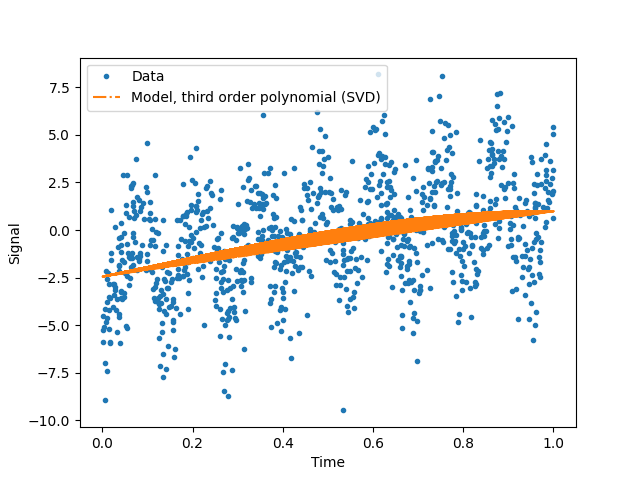
\includegraphics[width=0.7\textwidth]{t3.png}
    \caption{The thrid order polynomial is clearly not suited to fit the signal. This gives us no prediction power, and we have to improve the design matrix, A to include higher order terms in our model}. 
    \label{t3}
\end{figure}

Part C:
The residuals of the model against the data are shown in Figure \ref{res}

\begin{figure}[!htbp]
    \centering
    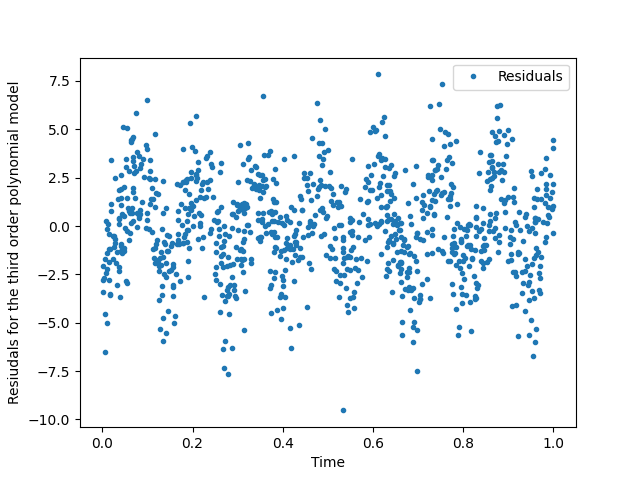
\includegraphics[width=0.7\textwidth]{residuals.png}
    \caption{The residuals are found to be significantly larger than that of the uncertainty of 2.0 in signal units. Unfortunately, we cannot learn much of the fit from the residuals.}
    \label{res}
\end{figure}

Part D:
We now try with a polynomial of order $n=20$ to see if that makes a better fit for our noisy data. The condition number is now: $9.1 \times 10^{14}$, which is a lot higher, meaning we are in the danger of overfitting. See Figure \ref{30}.
\begin{figure}[!htbp]
    \centering
    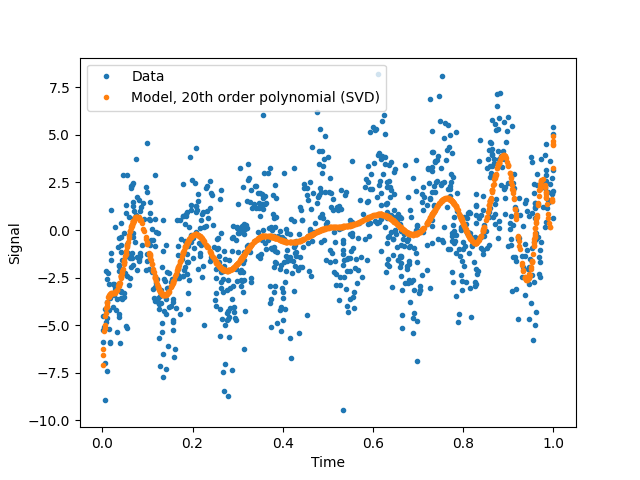
\includegraphics[width=0.7\textwidth]{model30.png}
    \caption{The fit is much better, since it captures the oscillatory behavior, but still not quite good enough at the beginning and end of the fit}.

    \label{30}
\end{figure}

Part E: 
We now try a Fourier series of order $n=18$, where the fit nicely follows that of the oscillations burried in the noise, as seen in Figure \ref{F}. The condition number is now $1.8 \times 10^{14}$.
\begin{figure}[!htbp]
    \centering
    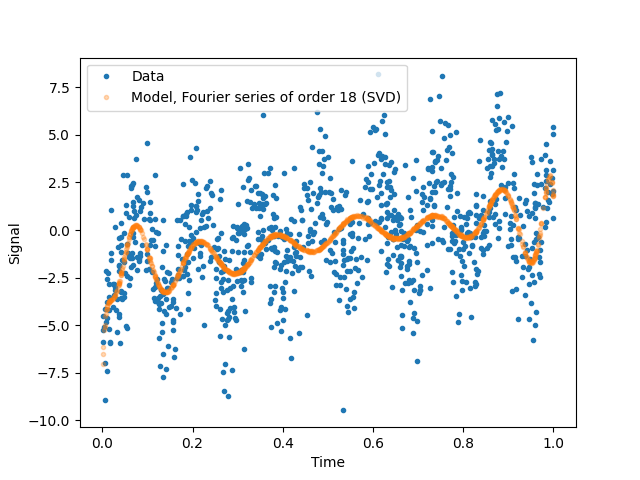
\includegraphics[width=0.7\textwidth]{fourier.png}
    \caption{The Fourier series fits the data at order $n=18$.}

    \label{F}
\end{figure}

From this fit we find the period in the scaled units to be around 0.15, which corresponds to around 5 years if the original time unit were in seconds. This could, likely, be the period of an exoplanet orbiting a distant star. 




\end{document}